\documentclass[10pt,a4paper]{article}
\usepackage[utf8]{inputenc}
\usepackage[ngerman]{babel}
\usepackage[T1]{fontenc}
\usepackage{amsmath}
\usepackage{amsfonts}
\usepackage{amssymb}
\usepackage{graphicx}
\usepackage{lmodern}
\usepackage{physics}
\usepackage[left=1cm,right=1cm,top=1.5cm,bottom=1.2cm]{geometry}
\usepackage{siunitx}
\usepackage{fancyhdr}
\usepackage{enumerate}
\usepackage{mhchem}
\usepackage{mathtools}
\usepackage{graphicx}
\usepackage{float}
\usepackage[table]{xcolor}
\usepackage{mdframed}
\usepackage{csquotes}
\usepackage{trfsigns}
\usepackage{capt-of}
\usepackage{adjustbox}
\usepackage{verbatim}

\sisetup{locale=DE}
\sisetup{per-mode = symbol-or-fraction}
\sisetup{separate-uncertainty=true}
\DeclareSIUnit\year{a}
\DeclareSIUnit\clight{c}
\mdfdefinestyle{exercise}{
	backgroundcolor=black!10,roundcorner=8pt,hidealllines=true,nobreak
}

\begin{document}
\twocolumn
\pagestyle{fancy}
% \lhead{DSV Formelsammlung, Stand {\input{\string"| date + " %Y-%d-%m" \string"}}}
\lhead{Formelsammlung Mathe, \today}
\rhead{Sedlmeier, Toni}
\section{Wahrscheinlichkeiten}
%%%%%%%%%%%%%%%%%%%%%%%%%%%%%%%%%%%%% Elementare System-Eigenschaften %%%%%%%%%%%%%%%%%%%%%%%%%%%%%%%%%%%%%%%%%%%%
  \subsection{Axiome von Kolmogoroff}
  \begin{enumerate}[(K1)]
      \item $P(A) \geq 0$ \ \ Nichtnegativität
      \item $P(\Omega) = 1$ \ \ Normierung
      \item Falls $A \cap B = 0 \rightarrow P(A\cap B)=P(A)+P(B) $ \ \ Additivität
  \end{enumerate}
  
  \subsection{Rechenregeln}
  \begin{mdframed}[style=exercise]
    \begin{align}
        P(A \cup B ) = P(A) + P(B) - P(A \cap B )
    \end{align}
  \end{mdframed}
    $A_1$ ... $A_n$ paarweise disjunkt (keine Scnittfläche)
  \begin{mdframed}[style=exercise]
    \begin{align}
        P(A_1 \cup A_2 \cup ... A_n) = P(A_1) + P(A_2) + ... +P(A_n)
    \end{align}
  \end{mdframed}
  falls nicht disjunkt Schnittfläche abziehen
  \begin{mdframed}[style=exercise]
    \begin{align}
        P(A \cup B ) = P(A) + P(B) - P(A\cap B)
    \end{align}
  \end{mdframed}
  
  \begin{mdframed}[style=exercise]
    \begin{align}
        P(A \cup B ) = 1 - P(\overline{A} \cap \overline{B})
    \end{align}
  \end{mdframed}


  \subsection{Bedingte Wahrscheinlichkeiten}
  \begin{mdframed}[style=exercise]
    \begin{align}
    P (A \cap B) = P (B) \cdot P (A\ |\ B).
    \end{align}
  \end{mdframed}

  \subsubsection{Baumdiagramm}
  \begin{center}
      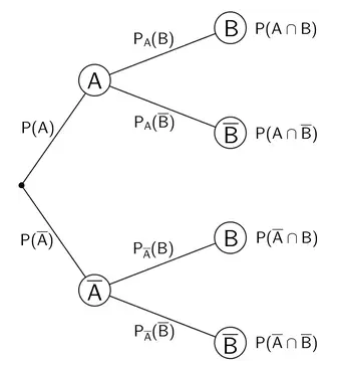
\includegraphics[width=.22\textwidth]{./img/baum.png}
  \end{center}
  \subsubsection{4-Felder Tafel}
  \begin{center}
      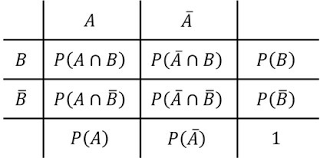
\includegraphics[width=.22\textwidth]{./img/vier.png}
  \end{center}

  \subsubsection{Stoch. Unabhängigkeit}
  \begin{mdframed}[style=exercise]
    \begin{align}
        P (A \cap B) = P(A) \cdot P(B)
    \end{align}
  \end{mdframed}

  \subsection{Satz von Bayes}
  \begin{mdframed}[style=exercise]
    \begin{align}
        P(A) = \displaystyle\sum_{i=1}^{n} P(A|B_i) \cdot P(B_i) \\
        P(B) = \displaystyle\sum_{i=1}^{n} P(B|A_i) \cdot P(A_i)
    \end{align}
  \end{mdframed}

  \begin{mdframed}[style=exercise]
    \begin{align}
        P (A_i \ |\ B) = \frac{P(A_i \cap B)}{P(B)} = \frac{P(B | A_i) \cdot P(A_i)}{P(B)}
    \end{align}
  \end{mdframed}

  \newpage

  \section{Diskrete Verteilungen}
  $E$ = Ereignis\\
  $\omega$ = Ergebnis\\
  $\Omega$ = Ergebnisraum\\

  Bsp: Würfeln
  \begin{center}
      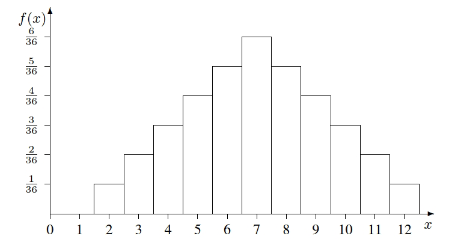
\includegraphics[width=.22\textwidth]{./img/wuerfel.png}
  \end{center}
Wahrscheinlichkeitsdichtefunktion $f_X(x)$ beschreibt die Wahrscheinlichkeit $P(X=x_i)$, 
dass die ZV $X$ den Wert $x_i$ annimmt
  \begin{mdframed}[style=exercise]
    \begin{align}
        f_X(x):=\left\{\begin{array}{ll} P(X=x_i) = p_i,  & x = x_i\in W(X) \\
         0, & sonst\end{array}\right. .
    \end{align}
  \end{mdframed}

\subsection{Erwartungswert}
  \begin{mdframed}[style=exercise]
    \begin{align}
        E(aX +b) &= aE(X)+b \\
        E(X \cdot Y) &= E(X) \cdot E(Y)\\
        E(X + Y) &= E(X) + E(Y)
    \end{align}
  \end{mdframed}

\subsection{Varianz}
  \begin{mdframed}[style=exercise]
    \begin{align}
        Var(aX) &= a^2 Var(X) \\
        Var(X + a) &= Var(X)  \\
        Var(X + Y) &=  Var(X) + Var(Y)\\
    \end{align}
  \end{mdframed}

  \begin{mdframed}[style=exercise]
    \begin{align}
        \mu_x &= E[x] = \displaystyle\int_{-\infty}^{\infty} \alpha f_x(\alpha) d\alpha = \displaystyle\sum_{\nu}^{} a_\nu P_\nu\\
        \sigma_x^2 &= E[(x-\mu_x)^2] = E[x^2]-\mu_x^2  = \displaystyle\int_{-\infty}^{\infty} (\alpha-\mu_x)^2 \ f_x(\alpha) d\alpha
    \end{align}
  \end{mdframed}
  
\subsection{Diskrete Gleichverteilung}
Alle Werte mit gleicher Wahrscheinlichkeit \\
\textbf{Wertebereich:} $W(X)= \{x_1 ... x_n \}$
  \begin{mdframed}[style=exercise]
    \begin{align}
        f_X(x):=\left\{\begin{array}{ll} \frac{1}{n},  & x \in W(X) \\
         0, & sonst\end{array}\right. .
    \end{align}
  \end{mdframed}

  \begin{mdframed}[style=exercise]
    \begin{align}
        E(X) &= \frac{1}{n} \sum_{i=1}^n x_i \\
        Var(X) &= \frac{1}{n} \sum_{i=1}^n x_i^2 
    \end{align}
  \end{mdframed}

\subsection{Bernoulli - Verteilung}
Zufallsprozess mit 2 möglichen Ausgängen (z.B Prüfungen) \\
\textbf{Wertebereich:} $W(X)= \{0;1 \}$\\
\textbf{Notation:} X $\sim$ Ber(p) mit p = P(A) 
  \begin{mdframed}[style=exercise]
    \begin{align}
        f_X(x):=\left\{\begin{array}{ll} P(X=0) = p_A \\
         P(X=1) = 1-p_A \end{array}\right. .
    \end{align}
  \end{mdframed}

  \begin{mdframed}[style=exercise]
    \begin{align}
        E(X) &= p \\
        Var(X) &= p(1-p) 
    \end{align}
  \end{mdframed}

\subsection{Binomial - Verteilung}
Zählen der Ereigniseintritte bei $n$ unabhängigen Bernoullivorgängen \\
\textbf{Wertebereich:} $W(X)= \{0 ... n \}$\\
\textbf{Notation:} X $\sim$ Bin(n,p) \\
\textbf{Parameter:} \begin{itemize}
    \item $p$ = WSK des Bernoullivorgangs 
    \item $n$ = Anzahl Wiederholungen 
    \item $x$ = Anzahl Ereigniseintritte 
\end{itemize}
  \begin{mdframed}[style=exercise]
    \begin{align}
        f_X(x):=\left\{\begin{array}{ll} \binom{n}{x} \cdot p^x \cdot (1-p)^{n-x}, & n \in W(X) \\ \\
        0, & sonst \end{array}\right. .
    \end{align}
  \end{mdframed}

  \begin{mdframed}[style=exercise]
    \begin{align}
        E(X) &= n\cdot p \\
        Var(X) &= n\cdot p (1-p) 
    \end{align}
  \end{mdframed}
  Additionseigenschaft:
  \begin{mdframed}[style=exercise]
    \begin{align}
        X   &\sim Ber(n,p)\\
        Y   &\sim Ber(m,p)\\
        X+Y &\sim Ber(n+m,p)
    \end{align}
  \end{mdframed}

\subsection{Poisson - Verteilung}
Anzahl an Ereigniseintritten in fixen Zeitintervallen \\
\textbf{Wertebereich:} $W(X)= \mathbb{N}$ \\
\textbf{Notation:} $X \sim Poi(\lambda)$ \\
\textbf{Parameter:} \begin{itemize}
    \item $\lambda$ = Rate
\end{itemize}

  \begin{mdframed}[style=exercise]
    \begin{align}
        f_X(x):=\left\{\begin{array}{ll} \frac{\lambda^x}{x!} e^{-\lambda}, & n \in W(X) \\ \\
        0, & sonst \end{array}\right. .
    \end{align}
  \end{mdframed}

  \begin{mdframed}[style=exercise]
    \begin{align}
        E(X) &= n\cdot p \\
        Var(X) &= n\cdot p (1-p) 
    \end{align}
  \end{mdframed}


\end{document}
